\documentclass[a4paper,12pt, doubleside]{report}
\usepackage[top=1in, bottom=1in, left=1.30in, right=1.30in]{geometry}
\usepackage[T1]{fontenc}
\usepackage[utf8]{inputenc}
\usepackage{lmodern}
\usepackage[italian]{babel}
\usepackage[hidelinks]{hyperref}
\usepackage{listings}
\usepackage{dirtree}
\usepackage{float}
\usepackage{listings}
\usepackage{graphicx}
\usepackage{titling}
\usepackage[font=small,labelfont=bf]{caption}
\usepackage{verbatim}
\usepackage{gensymb}

\lstset{
            basicstyle=\ttfamily
        }

\pretitle{%
  \begin{center}
  \Large
  \vspace*{-1.5in}
  
\includegraphics[]{logo_unife}\\[\bigskipamount]
}
\posttitle{\end{center}}

\title{\textbf{UNIVERSITÀ DEGLI STUDI DI FERRARA\\}
\bigskip
\textit{Corso di Laurea in Informatica}\\
\bigskip
\bigskip
\bigskip
\bigskip
\bigskip
\bigskip
\bigskip
\textit{\textbf{Impiego di Python e OpenRTK nella ricostruzione tomografica Cone-Beam CT.\\}}
\bigskip
\bigskip
\bigskip
\bigskip
\bigskip
\bigskip
\bigskip
\bigskip
\bigskip
\bigskip
\textbf{\underline{Relatore:}}
\hfill
\textbf{\underline{Laureando:}\thinspace\thinspace\thinspace} \\
\textit{Prof. Giovanni Di Domenico}
\hfill
\textit{Danny Lessio}
\bigskip
\bigskip
\bigskip
\bigskip
\bigskip
\bigskip
\bigskip
\bigskip
\bigskip
}


\date{Anno Accademico 2015 - 2016}
\begin{document}

    \maketitle
    \newpage

    \chapter*{Introduzione}
        \par
            <TODO>
            <
        		L'introduzione va ad esplicitare quanto indicato brevemente nel sommario.
        
        		Occorrerà quindi descrivere il problema studiato o il progetto elaborato, il perché lo si è affrontato, l'ambito di applicazione del progetto realizzato.
        
        		Dall'introduzione il lettore deve comprendere l'argomento della tesi e come il tesista ha affrontato lo studio della risoluzione del problema eventualmente evidenziando eventuali contributi originali soprattutto nella realizzazione di un progetto (si pensi ad esempio a librerie sw realizzate ad hoc per lo sviluppo di un software...).
        
        		Inoltre dall'introduzione il lettore deve poter verificare se possiede le conoscenze per ben interpretare i contenuti descritti oppure se gli è necessario intraprendere prima la lettura di tesi precedenti o di altra letteratura di riferimento.
        
        		E' bene riportare nell'introduzione il riferimento ai capitoli di cui si compone la tesi con una breve descrizione dei contenuti di ogni singolo capitolo senza esplicitare gli eventuali sottocapitoli/paragrafi che saranno indicati nell'indice.
        
        		Spesso l'introduzione è l'ultimo capitolo che viene scritto, sebbene sia il rpimo che si incontra nella lettura della tesi.
        	>
        \par
            Questa tesi tratta lo studio e l'utilizzo della libreria OpenRTK \cite{openrtk-website} basata su Insight Toolkit (ITK).\cite{itk-website}, la quale fornisce sia un insieme di tools basilari per poter eseguire efficientemente ricostruzioni tomografiche ( filtering, forward projection, backprojection ), sia un set di strumenti per poter eseguire il calcolo a livello multithreaded, sia su CPU che su GPU. Presenta inoltre delle interfacce I/O calibrate per un insieme limitato di CAT scanner attualmente in commercio.
    
        \par
            Per semplificarne l'utilizzo viene realizzato un package Python che si appoggia sia sulla libreria OpenRTK per eseguire le retroproiezioni sia su tools esterni come SimpleITK, una libreria più leggera rispetto ad Insight ToolKit per aiutare nella normalizzazione e conversione delle proiezioni in formato .MHA / .MHD.
            Il package è eseguibile a linea di comando, ed è facilmente estendibile per coprire anche eventuali evoluzioni della libreria OpenRTK.
    
        \par
            [TODO nella sezione X si fa Y etc bla di blabla, il secondo di blabla]
    
    \newpage
    \tableofcontents
    \newpage
    \chapter{Presentazione}
        \section{Breve Storia TAC}
            \par
                Per tomografia (dal greco \textit{témnó}, tagliare, o \textit{tómos}, nel senso di "strato", e \textit{gráphó}, scrivere) si intende la tecnica spettroscopica mirata alla rappresentazione a strati di un oggetto, in contrapposizione alla radiografia convenzionale la quale dispone sulla superficie bidimensionale della lastra tutto lo spessore del corpo o oggetto.\\
                La tomografia trova impiego soprattutto in medicina, ma anche in archeologia, geofisica, chimica e scienze dei materiali.
                
                <TODO questa parte iniziale non mi piace affatto>
                infatti puoi inserire una descrizione più dettagliata prelevando la roba da questo libro:
                \url{https://books.google.it/books?id=ba9yAgAAQBAJ&pg=PA202&lpg=PA202&dq=hounsfield+radon&source=bl&ots=rx7UNFYyba&sig=cs2Q6B3sy-LOMMffco3cttyVhxM&hl=it&sa=X&ved=0ahUKEwirqqOKhIrQAhULtBQKHVKsCTAQ6AEIMDAD#v=onepage&q&f=false}
                
               
            \subsection{Limiti della Radiografia Convenzionale}
                \par
                    Al fine di comprendere l'importanza della Tomografia Computerizzata, è importante comprendere le limitazioni imposte dalla radiografia convenzionale. Questa metodologia è sostanzialmente composta da una sorgente a raggi X, i quali vengono proiettati attraverso il corpo ed impressi su lastra radiografica bidimensionale. E’ essenzialmente il risultato dell’attenuazione media\cite{hounsfield-nobel-lecture} dei raggi dovuta alla composizione del materiale incontrato dalla sorgente alla pellicola. Nel caso in cui l’oggetto in esame sia il corpo umano, la quantità di attenuazione è direttamente proporzionale alla densità dei vari tessuti incontrati: i polmoni, contenendo aria, assorbono poca radiazione; le ossa, essendo molto dense, ne assorbono maggiormente.
                            
                    \begin{figure}[h]
                        \centering
                        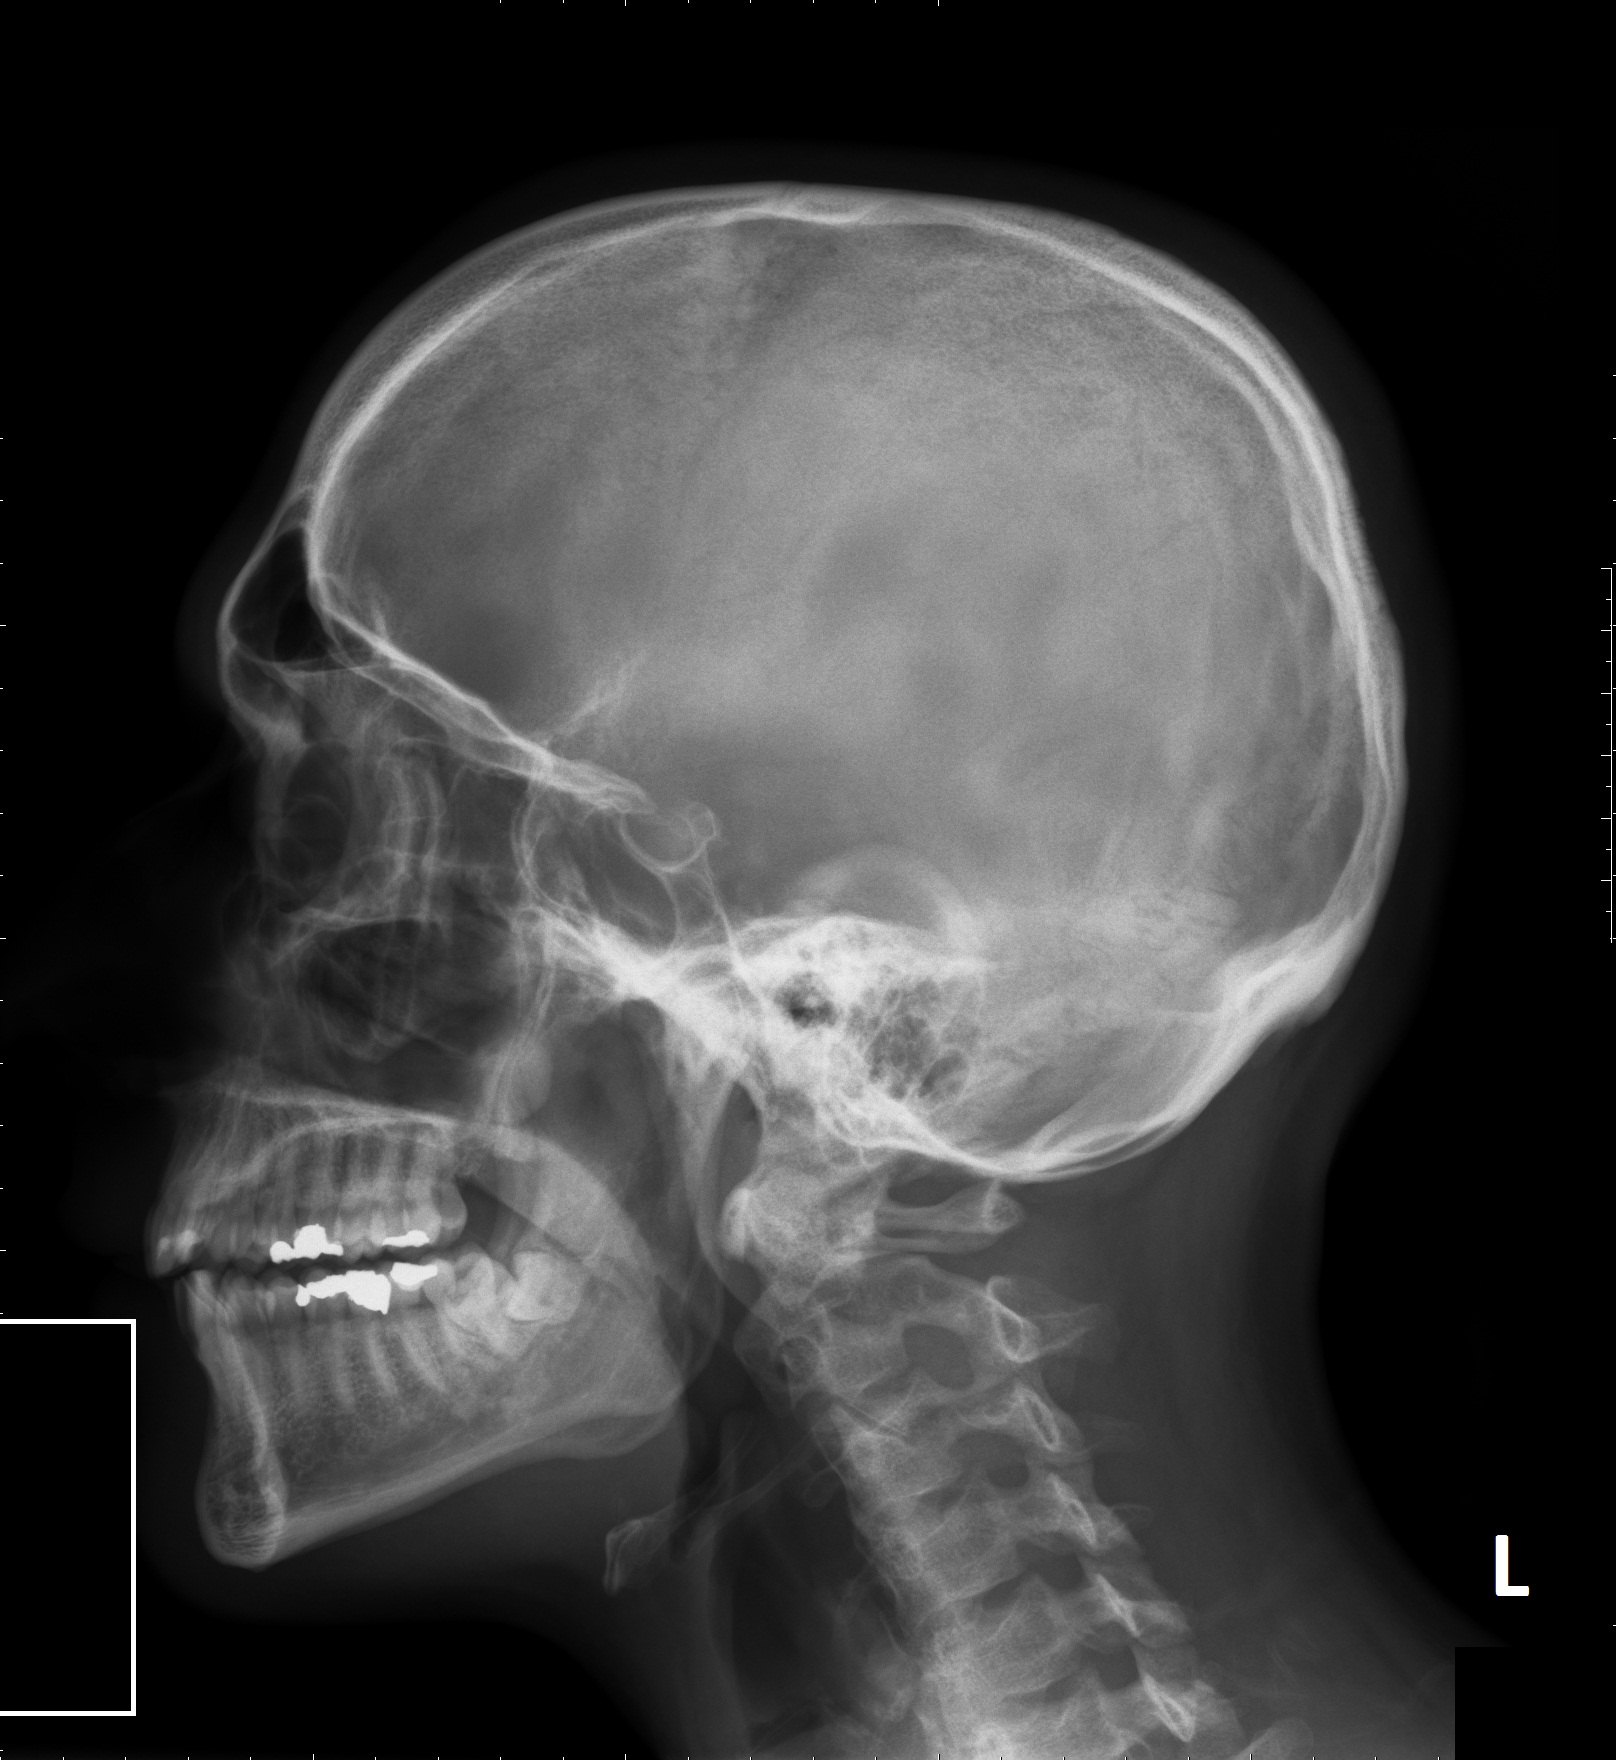
\includegraphics[width=0.4\textwidth]{radiografia}
                        \caption{Una radiografia al cranio - vista laterale.}
                        \label{fig:skull}
                    \end{figure}
                        
                    Dalla radiografia in \texttt{Figura \ref{fig:skull}}, è possibile distinguere solamente cinque vari livelli di densità. Partendo dal meno denso, si visualizza \textit{l'aria}, di colore nero; \textit{l'acqua o i tessuti molli}, che si visualizzano con un grigio chiaro; \textit{il grasso}, evidenziato con un colore grigio scuro; \textit{le ossa}, che presentano una colorazione tendente al bianco; \textit{il campione metallico} (L), di colore bianco.
                            
                    
                        <ASK> <TODO accertati che sia un campione metallico>
                        <TODO spiega cosa sono i tessuti molli>
                   
                            
                \par 
                    L’acqua ed i tessuti molli possiedono circa la medesima densità. Come si sarà notato in figura, è impossibile analizzare il cervello ed evidenziarne un'eventuale patologia, poiché esso è rappresentato come una zona omogeneamente grigia. L'ottenimento di un'immagine del cervello mediante radiografia classica rimase una sfida sin dal periodo immediatamente successivo al 1985, anno in cui vennero scoperti i raggi X. Anche il grande scienziato ed inventore Thomas Edison agli inizi del '900 si cimentò senza successo nell'impresa, a causa delle grosse limitazioni che l'analisi imponeva.\cite{thomas-edison-brain} Il cervello è infatti composto da tessuti molli, racchiusi all’interno di uno scheletro denso che impedisce alla maggior parte della radiazione di penetrarli, inoltre fluttua a bagno in un liquido chiamato \textit{fluido celebro spinale\footnote{Liquido che fornisce nutrienti ed agisce come cuscino al fine di proteggere la materia grigia stessa}} il che rende ancor più ardua l'impresa. Questo tipo di analisi, si scoprì, essere totalmente inaccessibile alla radiografia convenzionale.
                            
                \par
                    Un radiogramma impone diversi limiti diagnostici. Il \textit{problema delle ombre} è una diretta conseguenza del fatto che le complesse strutture tridimensionali del corpo umano, nella radiografia, vengono impresse su lastra bidimensionale. Un tumore, ad esempio, se fosse celato da una struttura ad alta densità come le costole, potrebbe passare completamente inosservato alla diagnosi. Questo fu il problema che tormentò i radiologi sin dagli inizi del XX secolo e, come si vedrà nella sezione 1.1.2, fu la ragione che portò allo sviluppo delle prime forme di tomografia classica (non computerizzata).
                    La lastra radiografica inoltre risulta un mezzo intrinsecamente inadeguato al fine di registrare le differenze di intensità dovute all'attenuazione dei raggi X durante il passaggio attraverso il corpo, questo non consente la distinzione tra tessuti molli.
                            
                \par
                    Il vero problema della radiografia convenzionale è dunque l'immensa perdita di informazione riscontrata in fase di acquisizione. Il \textit{problema delle ombre} verrà parzialmente risolto con lo sviluppo della tomografia convenzionale, l'analisi dei tessuti molli sarà invece possibile solamente con l'avvento della Tomografia Computerizzata (TC), che consentirà inoltre l'accurata misurazione dei valori d'assorbimento, riuscendo a differenziare la natura del materiale o del tessuto.
                            
            \subsection{Tomografia Convenzionale}
                \par
                    Per \textit{tomografia convenzionale} si intende l'ottenimento di un tomogramma <TODO spiega cos'è> senza l'ausilio di computazione. Questa tecnica venne completamente rimpiazzata con la Tomografia Computerizzata intorno al 1980.
                            
                \par
                    I primi studi risalgono al primo ventennio del 1900 e la tomografia convenzionale, curiosamente, venne indipendentemente scoperta più volte da diversi ricercatori sia Europei che Americani senza che questi scambiassero informazioni: all'epoca, i livelli di comunicazione non erano affatto sviluppati. Un pensiero espresso da Alessandro Vallebona, uno dei cinque grandi pionieri di questa metodologia, era il seguente: \textit{“quando un settore della scienza e della tecnica è maturo per progredire, per fare un passo avanti, il progresso avviene, a volte contemporaneamente oppure a breve distanza di tempo, promosso da persone diverse, anche in Paesi diversi”}\cite{vallebona-pensiero}.
                    Non è infatti difficile recuperare manoscritti nei quali si rivendicano la paternità dell'opera e violazioni d'utilizzo dei brevetti\cite{vallebona-difesa}. Queste ricerche indipendenti, produssero differenti nomenclature generando molta confusione riguardo l'oggetto di studio. Solamente nel 1962, durante la \textit{International Commission of Radiologic Units and Measurements} (ICRU\footnote{\url{http://www.icru.org/}}), venne selezionata la nomenclatura “tomografia”, che venne presto adottata ovunque nel Mondo.
                            
                \par
                    Come accennato in sezione 1.1.1, i ricercatori del primo ventennio del ‘900 condivisero uno scopo comune: escogitare un sistema che permettesse la separazione delle ombre registrate quando complesse strutture come il corpo umano venivano impressionate su lastra radiografica. Furono offerte numerose soluzioni ed il metodo più convincente risultò la stratificazione dei tessuti del corpo. In questo modo, utilizzando la geometria proiettiva, il problema delle ombre poteva essere parzialmente superato, nonostante gli ancora elevati livelli di radiazione richiesti dalla procedura.
                            
                    \begin{figure}[h]
                        \centering
                        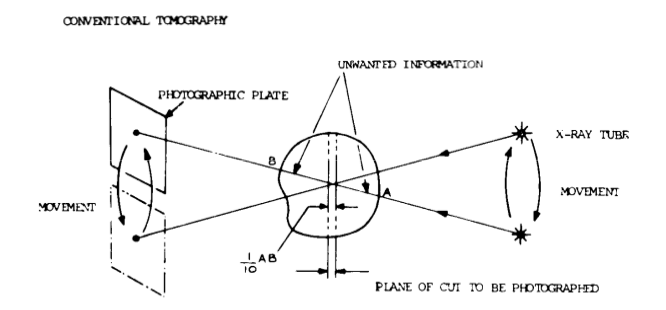
\includegraphics[width=0.8\textwidth]{conventional}
                        \caption{Principio di funzionamento della tomografia convenzionale.}
                        \label{fig:conventional}
                    \end{figure}
                            
                    Per poter eseguire la tomografia convenzionale senza computazione, in un puro sistema meccanico, due dei tre elementi (tubo, paziente e lastra) dovevano necessariamente muoversi in modo sincrono durante l’esposizione alla radiazione.
                    Per poter meglio comprendere il principio di funzionamento, si osservi la \texttt{Figura \ref{fig:conventional}} nella quale si mostra come fosse possibile ottenere una singola slice del corpo basandosi esclusivamente sui principi della geometria proiettiva. In questo caso il corpo (al centro) viene mantenuto fermo, mentre tubo e lastra si muovono in modo sincrono ed opposto. Si può notare che solamente circa 1/10 della lunghezza del fascio AB attraversa effettivamente il piano di interesse; i restanti 9/10 attraversano il corpo collezionando informazione inutile, non voluta. Questa è la motivazione per cui, in questi tomogrammi, era facile riscontrare artefatti\cite{hounsfield-nobel-lecture}.
    
                \par
                    André Edmund Marie Bocage, Alessandro Vallebona, Ziedses des Plantes, Gustav Grossmann e Jean Kieffer furono tra i primi ricercatori che contribuirono considerevolmente allo sviluppo di questa nuova metodologia. Bocage nel 1922 ottenne il primo brevetto; Vallebona realizzò diversi prototipi e contribuì alla letteratura con ben 370 pubblicazioni nelle scienze radiologiche\cite{vallebona-ricordo}; des Plantes è ritenuto il pioniere della sperimentazione; Grossmann contribuì all’analisi matematica del metodo e rese più snelli i progetti preesistenti; Kieffer fu il primo pioniere Americano, diede una descrizione esaustiva del suo dispositivo e alla matematica del sistema. I prototipi creati da questi pionieri vennero per lo più utilizzati a scopi di ricerca, l'utilizzo, se a fine clinico, non era affatto confortevole.
    
                \par
                    Lo sviluppo del primo dispositivo clinico per la tomografia convenzionale, il Polytome, venne sviluppato a Parigi nel 1950. Le immagini ricavate da questo dispositivo stimolarono le ricerche in ambito clinico, inizialmente dagli Europei e successivamente dagli Americani (anni ‘60).
                            
                    \begin{figure}[h]
                        \centering
                        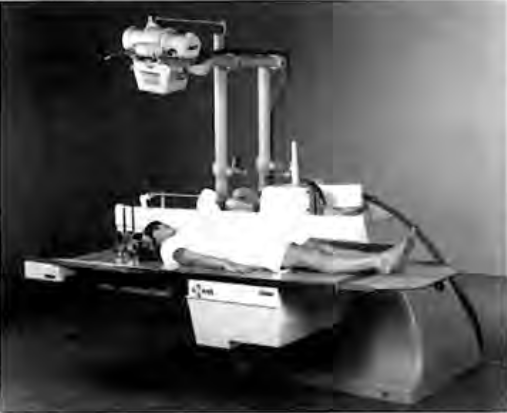
\includegraphics[width=0.5\textwidth]{polytome}
                        \caption{L'Universal Polytome, sviluppato a Parigi dalla Massiot-Philips.}
                        \label{fig:polytome}
                    \end{figure}
                        
                            
                    Le applicazioni più frequenti, riguardavano quelle parti del corpo in cui poteva essere presente un alto livello di contrasto, come il cranio. Queste immagini sezionali permettevano l’esplorazione dell’intricata rete ossea, tra cui i seni paranasali, la sella turcica\footnote{La sella turcica o sella turca costituisce la faccia superiore del corpo dell'osso sfenoide, un osso impari e mediano del neurocranio.} ed altre aree completamente inaccessibili alla radiografia convenzionale. Comparirono successivamente al Polytome diversi nuovi dispositivi che evidenziarono la necessità di ottenere un efficace imaging sezionale.
                \par
                    E’ importante notare che la tomografia convenzionale non permise l’accesso all’imaging dei tessuti molli, un’immagine sezionale del cervello risulterà quindi possibile solo con l’avvento della Tomografia Computerizzata. Si può storicamente affermare che la tomografia convenzionale ha gettato le basi al di sopra delle quali si sono evolute le avanzate tecnologie di imaging sezionale computerizzato che oggi apprezziamo.
                        
            \subsection{Nascita della TAC}
                \par      
                    La nascita della Tomografia Computerizzata riflette l'evoluzione della tomografia classica. Il pensiero di Vallebona, citato nella sezione 1.1.2, ha validità anche in questo caso: tre ricercatori, Allan McLeod Cormack, William H. Oldendorf e Godfrey N. Hounsfield, indipendentemente, svilupparono i principi base della TC intorno al 1960. Cormack ed Hounsfield ricevettero il Premio Nobel nel 1979, Oldendorf fu invece vittima di una controversia\cite{nobel-debate} e non venne premiato. 
                    Sia Cormack che Oldendorf ottennero prototipi funzionanti, ma l'ingegnere britannico Godfrey N. Hounsfield fu l'unico in grado di ottenere diverse realizzazioni commerciali di successo.
                \par
                    Hounsfield lavorò dal 1951 per la EMI Ltd di Londra, periodo nel quale si interessò particolarmente ai computer e contribuì alla costruzione del primo computer a transistor in assoluto assemblato in Gran Bretagna\cite{housfield-autobiografia}. Successivamente, negli anni '60, egli concepì l’idea della Tomografia Computerizzata ed iniziò le prime sperimentazioni.
                            
                    \begin{figure}[h]
                        \centering
                        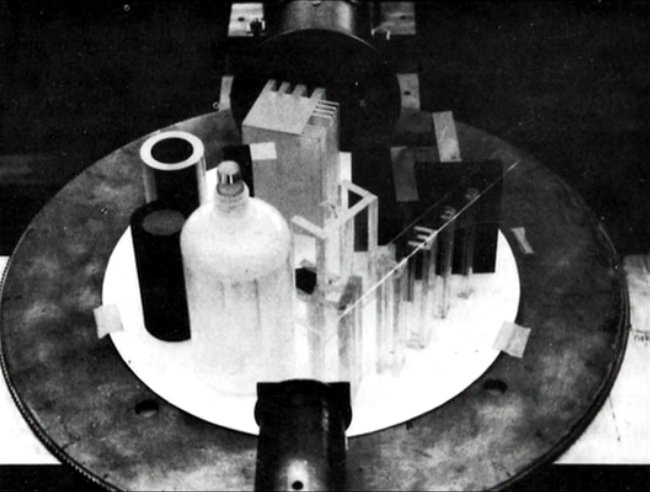
\includegraphics[width=0.5\textwidth]{first-prototype}
                        \caption{Il primo prototipo realizzato da Hounsfield}
                        \label{fig:prototype}
                    \end{figure}
                            
                    Il primo prototipo era composto da una scatola di piombo con un piccolo foro posto nella parte anteriore, all’interno della quale era presente un materiale radioattivo, l’Americium, capace di fornire una fonte costante, non particolarmente intensa, di raggi gamma. La radiazione fuoriusciva dal foro in singolo fascio collimato a configurazione pencil-beam. Il piatto visibile in \texttt{Figura \ref{fig:prototype}} veniva traslato orizzontalmente per permettere al singolo fascio di poter raggiungere tutti gli oggetti. Al termine della traslazione, il piatto veniva fatto roteare di 1\degree, ed il procedimento veniva ripetuto fino all'ottenimento di 180 <ASK accertati d'aver capito bene, cone beam? perchè 360?> <TODO spiega perchè 180> proiezioni. I livelli d'attenuazione erano letti dal signolo detector opposto alla sorgente. Il processo di scansione durò ben nove giorni, la ricostruzione\footnote{<TODO verrà trattata laggiu>} computerizzata degli oggetti richiese più di due ore di processamento. Questo fu un risultato molto importante, poiché dimostrò che la Tomografia Computerizzata era tecnologicamente e fisicamente possibile.
                    Hounsfield ed i suoi collaboratori, mantenendo la stessa geometria a rotazione-traslazione, continuarono lo sviluppo dei prototipi diminuendo sempre più il tempo di acquisizione. Si resero presto conto che l'avanzamento tecnologico avrebbe permesso l'analisi dei tessuti molli, ma non furono ancora certi che questo avrebbe permesso la localizzazione spaziale dei tumori. A verifica di ciò venne creato il primo dispositivo ad utilizzo clinico, molto più veloce e sofisticato rispetto ai prototipi precedenti, dedicato alla sola analisi del cranio, che doveva rimanere estremamente fermo durante la scansione.
                            
                    \begin{figure}[h]
                        \centering
                        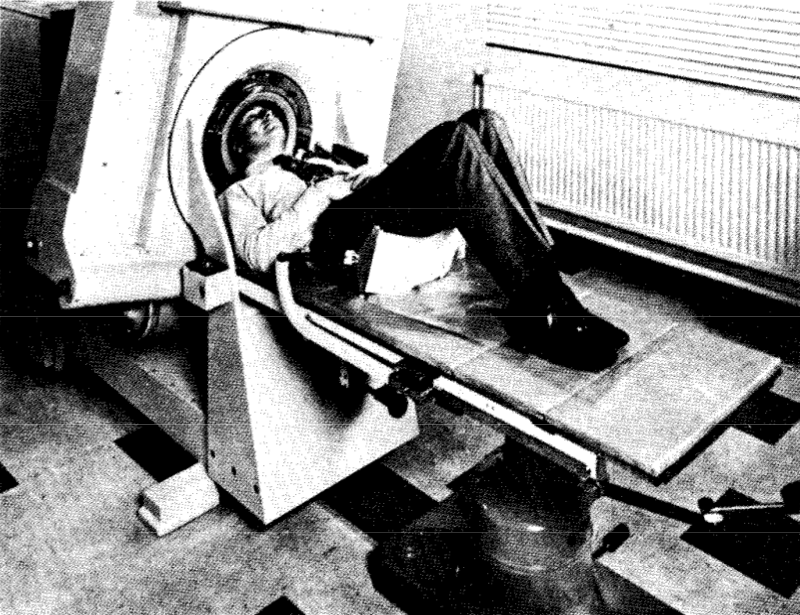
\includegraphics[width=0.5\textwidth]{clinical}
                        \caption{Il primo dispositivo ad utilizzo clinico installato all'Atkinson Morley’s Hospital di Londra.}
                        \label{fig:clinical}
                    \end{figure}
                            
                    Nel 1972 la prima paziente in assoluto fu una donna, il cui cervello si pensava presentasse anomalie. La prima immagine clinica ottenuta con il dispositivo in \texttt{Figura \ref{fig:clinical}} rivelò in chiaro ed inconfondibile dettaglio una cisti circolare nera situata nel lobo frontale della paziente, che fu successivamente operata con successo. Da quel momento in poi, furono analizzati molti altri pazienti e diventò palese che la macchina risultava perfettamente in grado di effettuare con accuratezza sia l'analisi dei tessuti molli sia la distinzione tra tessuti sani e malati\cite{hounsfield-nobel-lecture}.
                    Per la prima volta nella storia, i limiti imposti dalla radiografia convenzionale visti in sezione 1.1.1 risultarono completamente superati e si aprì la strada ad una rapida innovazione che coinvolse la riduzione dei tempi di esposizione e l'analisi di tutte le parti del corpo. Il team coordinato da Hounsfield già qualche anno dopo, riuscì a costruire macchinari sempre più complessi, con un tempo di acquisizione prossimo ai tre secondi.
                            
            \subsection{Evoluzione generazionale}
                \par
                    Per evoluzione generazionale si intende la sequenza temporale nel quale un particolare tipo di CT scanner, avente una ben precisa disposizione dei componenti e specifiche caratteristiche nei movimenti meccanici di base, è stato introdotto nel mercato. E’ importante notare, che al crescere del numero di generazione non crescono necessariamente le performance del sistema.
                        
                \bigskip
                \par
                    \textbf{Scanner di prima generazione.} Come mostrato in \texttt{Figura \ref{fig:first-generation}}, la sorgente veniva collimata in un raggio pencil-beam direzionato ad un singolo detector allineato alla sorgente e posizionato all’altro lato degli oggetti. Una singola proiezione veniva ottenuta muovendo il tubo sorgente ed il detector in una traslazione. Per poter ottenere la successiva proiezione, l’intera struttura ruotava di 1\degree e veniva traslata nella direzione opposta. Questo processo, di rotazione e traslazione, doveva essere ripetuto fino all’ottenimento di 180 proiezioni. Le prime versioni richiedevano circa 4.5 minuti per poter portare a termine la scansione, ed erano limitate a quelle parti del corpo dove il movimento del paziente poteva essere controllato (testa). Questa particolare configurazione viene anche detta "\textit{parallel-beam}".
                            
                    \begin{figure}[h]
                        \centering
                        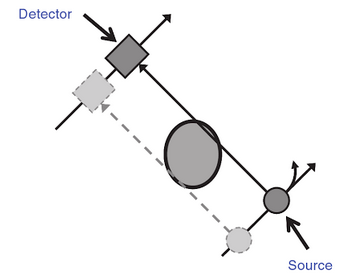
\includegraphics[width=0.5\textwidth]{first-generation}
                        \caption{Rappresentazione schematica di uno scanner di prima generazione.}
                        \label{fig:first-generation}
                    \end{figure}
                            
                \bigskip
                \par
                    \textbf{Scanner di seconda generazione.} Il maggiore sforzo per il miglioramento fu concentrato nella riduzione dei tempi di acquisizione, fino al punto di poter ottenere l’imaging di sezioni come il tronco. Aggiungendo detectors disposti angolarmente, diverse proiezioni potevano essere ottenute in una singola traslazione. Una delle prime applicazioni, ad esempo, che presentava 3 detectors con displacement di 1\degree, poteva effettuare 60 traslazioni anzichè 180. Questo era dovuto al fatto che ciascun detector vedeva la sorgente ad un angolo differente, ottenendo in una singola traslazione ben 3 proiezioni. Il sistema, una volta terminata la traslazione, poteva roteare di 3\degree  ed ottenere la nuova proiezione. I tempi di scansione erano quindi ridotti di un terzo. 
                        
                \bigskip
                \par
                    \textbf{Scanner di terza generazione.} In questi scanner, la sorgente è collimata in una struttura a ventaglio (fan-beam) diretta verso i detector disposti ad arco. Durante la scansione, il tubo e l’array di detector ruotano lungo il paziente e differenti proiezioni sono attenute durante la rotazione facendo pulsare la sorgente a raggi X oppure campionando i detector ad una frequenza elevata. Il sistema puramente rotazionale ha permesso l’accesso a sorgenti a più elevata potenza, permettendo una notevole riduzione dei tempi d’acquisizione. Un aspetto di questa geometria è che i raggi in una singola proiezione sono divergenti anziché paralleli. La divergenza dei raggi richiede qualche modifica all’interno degli algoritmi di ricostruzione. Tutti gli scanner CT odierni sono basati su modifiche di questo design. I tempi di acquisizione sono dell’ordine di pochi secondi e le recenti versioni riescono a scendere sotto al secondo.
                            
                    \begin{figure}[h]
                        \centering
                        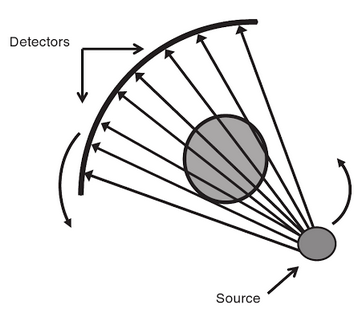
\includegraphics[width=0.5\textwidth]{third-generation}
                        \caption{Rappresentazione schematica di uno scanner di terza generazione.}
                        \label{fig:third-generation}
                    \end{figure}
    
                \bigskip
                \par
                    \textbf{Scanner di quarta generazione.} Questo particolare design si evolse simultaneamente alla terza generazione. In questo particolare caso, viene fatta roteare solo la sorgente e si ha un intero anello composto da detector. Inizialmente questi dispositivi possedevano 600 detector, successivamente arrivarono fino a 4800, con tempi di acquisizione comparabili agli scanner di terza generazione. Questo design tuttavia ha presentato diverse limitazioni, una tra queste è dovuta all’inefficiente utilizzo dei detector (meno di 1/4 è effettivamente utilizzato ad ogni istante della scansione). L'altra limitazione è dovuta ad una maggior suscettibilità alla presenza di artefatti (dovuti allo scattering). Per queste ragioni questi scanner non sono più commercialmente disponibili.
                            
                    \textbf{Scanner ad elica.} La tecnica coinvolge la continua acquisizione di proiezioni attraverso l’intero volume del paziente. La procedura viene eseguita roteando continuamente la sorgente ed i detector accompagnando il movimento del paziente in una traslazione all’interno del gantry\footnote{TODO footnote gantry}. Per poter ottenere un applicazione funzionante di questo tipo sono necessarie tre tecnologie: la \textit{Slip-Ring Technology}\footnote{Architettura composta da anelli conduttivi elettromeccanici che permettono al frame di scansione di poter roteare continuamente, senza doversi preoccupare dei cavi.}, tubi a raggi X ad elevata energia ed algoritmi di interpolazione che gestiscano le proiezioni non complanari. E’ una tecnologia molto importante perchè per la prima volta nella storia permette la scansione dell’intero corpo del paziente in tempi brevissimi.
    
                    \begin{figure}[h]
                        \centering
                        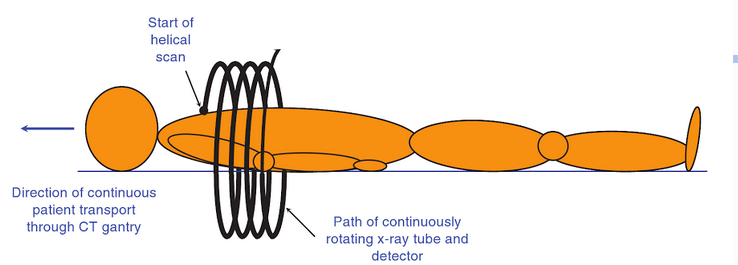
\includegraphics[width=0.5\textwidth]{helix}
                        \caption{Rappresentazione schematica di uno scanner ad elica.}
                        \label{fig:helix}
                    \end{figure}
                                            
        \section{Principi di Funzionamento TAC}
            \subsection{Proiezione}
            \subsection{Filtering}
            \subsection{Ricostruzione}
                <TODO>
                In questa sezione puoi pigliare l'introduzione di questo libro:
                \url{https://books.google.it/books?id=pqSNAgAAQBAJ&pg=PA35&lpg=PA35&dq=%22radiant+energy+apparatus+for+investigating+selected+areas+of+interior+objects+obscured+by+dense+material&source=bl&ots=tvcx6PeTbo&sig=IjYEBPukA9hr7Wrt9RTAekVzbjU&hl=it&sa=X&ved=0ahUKEwiS3JuF4Y7QAhUKbhQKHSMKCUoQ6AEIKjAD#v=onepage&q=%22radiant%20energy%20apparatus%20for%20investigating%20selected%20areas%20of%20interior%20objects%20obscured%20by%20dense%20material&f=false}
           
            
        \section{Principali Architetture TAC}
            \subsection{Cone Beam}
            \subsection{A spirale}
            \subsection{Ad emissione}
        
        
        \section{OpenRTK}
            \subsection{Storia del progetto}
                \par 
                    Il progetto nacque nel Giugno 2010 quando i founder Simon Rit e Gregory Sharp discussero riguardo la scarsità di soluzioni open-source nell'ambito della Cone-Beam CT. Infatti, l'unica alternativa presente era una libreria chiamata Plastimatch, la quale poteva già effettuare retroproiezioni filtrate sia su CPU che su GPU, ma l'architettura del software non teneva conto dell'evoluzione verso nuove tipologie di algoritmi iterativi. Decidettero quindi di dar vita ad una nuova piattaforma basata su Insight ToolKit (ITK), una libreria di elaborazione delle immagini già famosa all'epoca.
                \par
                    Gli sviluppi iniziali furono basati su codici preesistenti, la piattaforma permise in breve tempo l'ottenimento di ricostruzioni FBP utilizzando dati provenienti da diversi scanner commerciali CBCT. Questi sviluppi attirarono l'interesse dell' Université Catholique di Louvain, Francia e dell'azienda Beam Application (IBA) che stava sviluppando il primo scanner CBCT a protoni. RTK è ora utilizzato negli scanner IBA. Al giorno d'oggi questi partners sono riuniti sotto l'RTK Consortium. La piattaforma RTK fornisce una piattaforma efficiente per sviluppi continuativi, beneficiando costantemente delle nuove features di ITK.
                \par
                
                    Attualmente ( Novembre 2016 ) il Progetto viene mantenuto e sviluppato sulla piattaforma GitHub con circa 20 sviluppatori attivi.
                
                
            \subsection{Geometria}
                \par
                    <ASK come è composta veramente? necessito dello standard IEC? devo creare delle immagini che illustrino la configurazione geometrica?> <TODO>
                    RTK necessita di informazioni relative alla geometria di acquisizione per poter correttamente ricostruire un set di proiezioni. L'unica geometria configurabile è \texttt{ ThreeDCircularProjectionGeometry}, implementato come classe in RTK.
                    Lo scopo di questa classe è quella di definire un set di proiezioni 2D, acquisite mediante un detector bidimensionale lungo una traiettoria circolare. La descizione della geometria è basata nello standard internazionale IEC 61217 che è stato progettato per dispositivi cone-beam su sistemi isocentrici. Il sistema a coordinate fisse di RTK ed il sistema di coordinate fisse dell'IEC 61217 sono esattamente eguali. 
                    
                    9 parametri vengono utilizzati per ciascuna proiezione per definire la sorgente ed il detector relativi ad un sistema di coordinate fisso. I 9 parametri vengono settati con il metodo AddProjection. Vengono utilizzati dei valori di default per tutti quei parametri non esplicitamente espressi.
                        
                    const double sid, const double sdd, const double gantryAngle, const double projOffsetX=0., const double projOffsetY=0., const double outOfPlaneAngle=0., const double inPlaneAngle=0., const double sourceOffsetX=0., const double sourceOffsetY=0.
                        
                    The projection offset is the offset of the image origin from the
                    detector origin (the orthogonal projection of the isocenter on the
                    detector). But as I said, in many normal 2D image
                    format like .png, .tif, and .bmp, the image origin is not defined, and
                    ITK/RTK uses the first pixel as the image origin.
                    Then, there is another mapping from the image coordinate system to the
                    detector coordinate system. I have already explained the relationship
                    between the image origin and the detector origin above. How the image
                    axis (u and v) orientated with regard to the detector axis (x and y)
                    depends on the direction cosines of the image. Again, this information
                    does not exist in many 2D image format and the default value in
                    ITK/RTK is an identity matrix, so u/v and x/y are also aligned.\cite{rtk-users-proj-offset}
                
            \subsection{Ricostruzione rtkfdk}

        \section{SimpleITK}
            \subsection{Storia del progetto}
            \subsection{Wrapper Python}
                
        \section{Linguaggio Python}
            
        \section{Normalizzazione delle Proiezioni}
            \label{sec:normalizzation}
            \par
                L'intensità dei pixel componenti una proiezione, diretto risultato d'acquisizione da parte del detector, è direttamente proporzionale all'intensità della sorgente. Gli algoritmi di ricostruzione richiedono, per ogni proiezione, l'informazione relativa alla somma dei coefficienti di attenuazione lineare degli n voxel dell'oggetto attraversati durante l'acquisizione, informazione indipendente dall'intensità del fascio sorgente. La \textit{Normalizzazione dello Stack} non è altro che il processo di ottenimento della somma dei coefficienti di attenuazione a partire dalla rilevazione del detector.
            \par
                Per poter meglio comprendere gli effetti di questo procedimento, si osservi il seguente esempio:
                
                \begin{figure}[h]
                    \centering
                    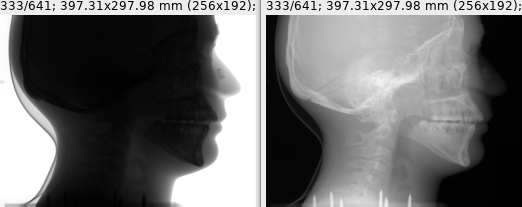
\includegraphics[width=0.7\textwidth]{normalization}
                    \caption{Effetti della procedura di normalizzazione. Immagine a sinistra: non normalizzata. Immagine a destra: normalizzata.}
                    \label{fig:skull-phantom}
                \end{figure}
                
                L'immagine a sinistra è la proiezione numero 333 su 641 acquisita dal detector. Come si può notare, l'oggetto presenta una colorazione molto scura
                <ASK perchè l'oggetto presenta una colorazione scura?> <TODO>
                
            
            \subsection{Aspetto Matematico}
                \label{sub:norm-math}
                \par
                    Le proiezioni appartenenti ad uno Stack, essendo il diretto risultato rilevato dal detector in fase di acquisizione, contengono l'informazione relativa all'attenuazione del fascio dovuta al passaggio attraverso il corpo. Ogni pixel di ciascuna proiezione (ottenuta ad un preciso angolo di acquisizione) registra l'intensità attenuata I, la quale è governata dalla legge di Lambert-Beer\cite{lambert-beer}:

                    \begin{equation} \label{eq:lambert}
                        \texttt{I} = \texttt{Io} \cdot e^{- (\mu1 + \mu2 + ...  + \mu n)}
                    \end{equation}
                    
                    Dove:
                    \begin{itemize}
                      \item \texttt{I} = Intensità rilevata (attenuata).
                      \item \texttt{$ (\mu1 + \mu2 + ... + \mu n) $} = Somma dei coefficienti di attenuazione lineare appartenenti ad n voxel incontrati.
                    \end{itemize}
                    
                \par
                    Avendo a disposizione l'intensità della sorgente \texttt{Io}, è possibile ottenere la somma dei coefficienti di attenuazione lineare manipolando algebricamente (\ref{eq:lambert}):
                    
                    \begin{equation} \label{eq:normalization}
                        (\mu1 + \mu2 + ... + \mu n) = - \log_e{(I/Io)}
                    \end{equation}
                    
                    Questo processo viene definito Normalizzazione delle proiezioni.
                
            \subsection{Ottenimento Io}
                \label{sub:io}
                \par
                    La sorgente non emette sempre la medesima intensità in ogni fase di acquisizione. Per questo motivo il valore \texttt{Io} dev'essere registrato o calcolato per ciascuna proiezione componente lo Stack (per ogni angolo di acquisizione).
                    Esistono due principali metodologie per poter ottenere questo valore:
               
                    \begin{enumerate}
                        \item Approssimazione:
                            \par
                                Se la dimensione dell'oggetto non ricopre l'intera area del detector, alcune zone del detector assorbono radiazione non attenuata.
                                
                                Per poter approssimare l'effettiva intensità della sorgente, è possibile selezionare il pixel avente l'intensità maggiore. Altre tecniche prevedono un calcolo basato sulla media dei pixel che non hanno registrato attenuazione.
                                E' da notare che questa tecnica non è sempre attuabile: nel caso in cui l'oggetto occupi l'intera area del detector, questo non conterrà aree non attenuate.
                        
                        \item Salvataggio Fisico:
                            \par
                                Un sensore posto in prossimità della sorgente sorgente registra l'intensità del fascio per quel particolare angolo prima che la radiazione attraversi l'oggetto. Questa alternativa è ideale poichè, oltre ad essere sempre attuabile, fornisce un'intensità \texttt{Io} sempre corretta (non approssimata).
                    \end{enumerate}                
                
                   
                    
                    
                                  
    \chapter{Sviluppo del Progetto}
        \section{Obiettivo}
            <TODO>
            Lo scopo principale del progetto riguarda la comprensione di OpenRTK come poter ottenere da questo una ricostruzione delle proiezioni a disposizione.
            Nonostante RTK sia originariamente scritto in C++, presenta un interfaccia wrapping nominata SimpleRTK. Nella descrizione della geometria, verrà trattata l'interfaccia OpenRKT.
         
        \section{Gli Stack di Proiezione a disposizione}
            <TODO>
            <ASK descrivo anche la conversione da .RAW ad .MHA? questo implica una descrizione approfondita di imagej?>
            La Facoltà ha messo a disposizione una decina di stack di proiezione, i quali presentavano le medesime caratteristiche. Originariamente composte in formato .RAW, sono stati convertiti mediante un estensione di ImageJ in immagini .MHA, per poterne favorire la lettura da parte di RTK. Uno stack era inoltre accompagnato da informazioni aggiuntive sull'apparato di acquisizione (SID, SDD, etc) inserite in un semplice file di testo. Per ogni proiezione appartenente ad un particolare stack era inoltre presente un file in formato .csv contenente informazioni riguardanti il preciso angolo di acquisizione, eventuali offset e l'intensità della sorgente non attenuata.
            Tutte le distanze erano espresse in millimetri.
            
            \subsection{Informazioni sull'acquisizione}
                \label{sub:acq_file}
                \par
                    Queste informazioni erano presenti su un file di testo esterno, in quanto riguardano esclusivamente l'apparato di acquisizione. 
                    
                    \begin{itemize}
                        \item SID/SDD: Stanno per \textit{Source to Isocenter Distance} e \textit{Source to Detector Distance}. L'isocentro è l'asse di rotazione del gantry\footnote{Termine tecnico che sta ad indicare il sistema rotazionale composto dall'accoppiata sorgente-detector.}.
                        \item Detector Size: Specificata come coppia di valori relativi alle direzioni (u,v). Rappresentano il numero di pixel che si trovano in ciascuna direzione. Questa informazione può essere anche ricavata osservando la dimensione in pixel di una proiezione: una proiezione non è nient'altro che l'informazione letta dal detector, ha dunque la medesima dimensione.
                        \item Pixel Detector Size: Specificata come una coppia di valori per entrambe le direzioni (u,v), sta ad indicare la dimensione di un singolo pixel del detector in millimetri.
                    \end{itemize}
                    
                    
            
            \subsection{Composizione File .csv}
                \label{sub:csv}
                <ASK accertati iso u iso v> <TODO>
                \par
                    Le proiezioni a nostra disposizione erano affiancate ad un file .csv il quale, per ogni riga, conteneva le seguenti informazioni:
                    \begin{lstlisting}[language=bash, frame=bt]
+-----------+-------+-------+-------+----+
| proj_name | angle | iso_u | iso_v | Io |
+-----------+-------+-------+-------+----+
                    \end{lstlisting}
                    
                    \begin{itemize}
                        \item \texttt{proj\textunderscore name}: Nome del file contenente tale proiezione;
                        \item \texttt{angle}: Angolo nel quale è stata acquisita la proiezione;
                        \item \texttt{iso\textunderscore u}:  Allineamento del detector alla sorgente. Nel caso in cui questi siano allineati, questo corrisponde esattamente a:
                        \newline
                        Detector\textunderscore Size\textunderscore u / 2 + 0.5
                        \newline
                        Esempio in \texttt{Figura \ref{fig:iso}}.
                        \item \texttt{iso\textunderscore v}: Allineamento del detector alla sorgente. Nel caso in cui questi siano allineati, questo corrisponde esattamente a:
                        \newline
                        Detector\textunderscore Size\textunderscore v / 2 + 0.5
                        \newline
                        Esempio in \texttt{Figura \ref{fig:iso}}.
                        \item \texttt{Io}: Intensità del fascio sorgente, non attenuato, registrato in fase di acquisizione. 
                    \end{itemize}
                    
                    \begin{figure}[h]
                        \centering
                        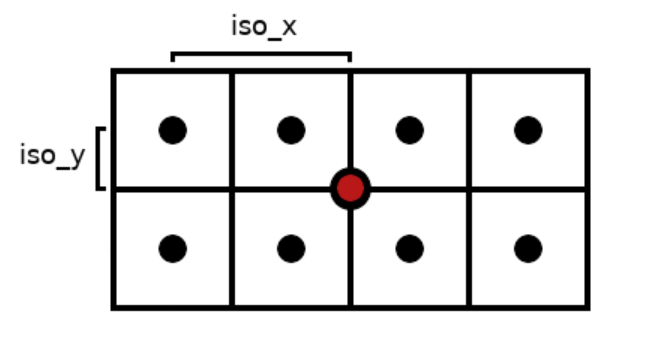
\includegraphics[width=0.6\textwidth]{iso}
                        \caption{In questa proiezione sorgente e detector sono allineati: Detector\textunderscore size\textunderscore x = 4 ; Detector\textunderscore size\textunderscore y = 2. Iso\textunderscore u = 2.5 ; Iso\textunderscore v = 1.5. In questo caso Iso\textunderscore u ed Iso\textunderscore v identificano il punto centrale. }
                        \label{fig:iso}
                    \end{figure}
                    
                    Le prime 4 informazioni verranno utilizzate al fine di generare il file di geometria per RTK. L'ultima informazione (Io) verrà utilizzata per effettuare la normalizzazione delle proiezioni. Il numero di righe del file .csv è pari al numero di proiezioni esistenti nello Stack.
                    
            \subsection{Composizione Stack .mha} 
                <TODO>
                <ASK sono necessari tutti i token?>
          
            
        \section{Configurazione OpenRTK e SimpleRTK}
            \subsection{Complilazione ITK}
                \par
                    La procedura di compilazione reperibile al sito \url{wiki.openrtk.org} soffre di alcuni mancati accorgimenti che non rendono chiara la procedura e la rendono onerosa in termini di tempo. L'intera procedura è stata automatizzata in uno script bash immediatamente accettato dalla comunity OpenRTK ed inserito nella wiki ufficiale
                    \cite{wiki-rtk}. Descriverò quindi la personale configurazione utilizzata all'interno dello script, visualizzabile nei listati <TODO>.
                \par    
                    RTK dipende direttamente da ITK, che dev'essere compilato e configurato manualmente. 
                    Inizialmente è necessario procurarsi i sorgenti da repository git mediante la procedura clone :
                    \begin{lstlisting}[language=bash, frame=bt]
$ git clone http://itk.org/ITK.git
                    \end{lstlisting}
                    
                    \bigskip
                    Si crea ora un nuovo direttorio, ITK-bin, e ci si posiziona all'interno di questo :
                    \begin{lstlisting}[language=bash, frame=bt]
$ mkdir ITK-bin
$ cd ITK-bin
                    \end{lstlisting}
                    
                    \bigskip
                    Mediante il comando \texttt{cmake} si abilitano/disabilitano i moduli desiderati:
                    
                    \begin{lstlisting}[language=bash, frame=bt]
$ cmake -DModule_ITKReview=ON -DITK_USE_FFTWD=ON 
-DITK_USE_FFTWF=ON -DBUILD_DOCUMENTATION=OFF 
-DBUILD_EXAMPLES=OFF -DBUILD_TESTING=OFF 
-DCMAKE_CXX_FLAGS=-fPIC -DCMAKE_C_FLAGS=-fPIC ../ITK
                    \end{lstlisting}
                    
                    I seguenti moduli sono direttamente richiesti da RTK:
                    \begin{itemize}
                        \item Module\textunderscore ITKReview
                        \item ITK\textunderscore USE\textunderscore FFTWD
                        \item ITK\textunderscore USE\textunderscore FFTWF
                    \end{itemize}
                    
                    Questi sono stati disabilitati al fine di permettere una più rapida compilazione:
                    
                    \begin{itemize}
                        \item BUILD\textunderscore DOCUMENTATION
                        \item BUILD\textunderscore EXAMPLES
                        \item BUILD\textunderscore TESTING
                    \end{itemize}
                    
                    Infine i seguenti flag, attivati sia per il compilatore C che per il compilatore CXX, riguardano la produzione di codice position-indipendent-code (PIC). Questo permette ad altre librerie, come SimpleITK, si poter sfruttare ITK come libreria condivisa. Per maggiori informazioni è possibile consultare \texttt{man gcc}. 
                    
                    \begin{itemize}
                        \item CMAKE\textunderscore CXX\textunderscore FLAGS = -fPIC
                        \item MAKE\textunderscore C\textunderscore FLAGS = -fPIC
                    \end{itemize}
                    
                    \bigskip
                    A questo punto è possibile compilare ITK, utilizzando il seguente comando:
                    \begin{lstlisting}[language=bash, frame=bt]
$ make -j
                    \end{lstlisting}
                    
                    L'opzione "-j", permette di specificare il numero di job eseguibili in parallelo durante la compilazione. Nel caso in cui non venga specificato il numero (come in questo caso), il sistema eseguirà quanti più job possibili in parallelo. Nel caso in cui questo comando venga eseguito su MS-DOS, questa opzione non avrà alcun effetto, in quanto il multi-processing non è supportato.\cite{-j-gnu-docs}. Questa particolare opzione non è inserita nel wiki di OpenRTK, se omessa può comportare diverse ore di computazione.
                    
                    Ora che ITK è compilato con successo, ci si riposiziona alla root del progetto:
                    \begin{lstlisting}[language=bash, frame=bt]
$ cd ..
                    \end{lstlisting}
            
            \subsection{Complilazione RTK}
                \par
                    È ora possibile procedere con la compilazione di RTK.
                    Per prima cosa si salva su variabile \texttt{path\textunderscore of\textunderscore ITK} il full path di ITK-bin che occorrerà successivamente. Il comando \texttt{pwd} è adatto allo scopo, in quanto recupera il path del direttorio corrente:
                    \begin{lstlisting}[language=bash, frame=bt]
$ cd ITK-bin
$ path_of_ITK=$(pwd)
$ cd ..
                    \end{lstlisting}
                    
                    A questo punto si recuperano i sorgenti di RTK, mediante lo stesso procedimento visto per ITK:
                    
                    \begin{lstlisting}[language=bash, frame=bt]
$ git clone http://github.com/SimonRit/RTK.git
                    \end{lstlisting}
                    
                    \bigskip
                    Si crea il direttorio RTK-bin e vi si entra:
                    \begin{lstlisting}[language=bash, frame=bt]
$ mkdir RTK-bin
$ cd RTK-bin
                    \end{lstlisting}
                    
                    Ora, attraverso cmake, si abilitano i moduli necessari e si effettua il link con ITK-bin:
                    \begin{lstlisting}[language=bash, frame=bt]
$ cmake -DITK_DIR=$path_of_ITK 
-DCMAKE_BUILD_TYPE=Release -DBUILD_EXAMPLES=ON 
-DCMAKE_CXX_FLAGS=-fPIC  -DCMAKE_C_FLAGS=-fPIC 
../RTK
                    \end{lstlisting}
                   
                    Come si può vedere il full path del direttorio ITK-bin è stato inserito nella variabile \texttt{ITK\textunderscore DIR}, è stata scelta la versione \texttt{Release} e sono state attivate, come per ITK, le direttive PIC.
    
                    A questo punto è possibile procedere con la compilazione:
                    \begin{lstlisting}[language=bash, frame=bt]
$ make -j
                    \end{lstlisting}
                   
                    Si ritorna nella root del progetto ed il processo di complizazione è terminato.
                    \begin{lstlisting}[language=bash, frame=bt]
$ cd ..
                    \end{lstlisting}
                    
                    Per poter controllare se il procedimento è andato a buon fine, è possibile lanciare l'eseguibile \texttt{HelloWorld} all'interno di RTK-bin/bin, il quale stamperà a video la stringa \texttt{"RTK Hello World!"}
                    \begin{lstlisting}[language=bash, frame=bt]
$ ./RTK-bin/bin/HelloWorld
                    \end{lstlisting}
                    
            \subsection{Configurazione Wrapping SimpleRTK}
                \par
                    Questa procedura non è stata fornita di script bash. Dalla root directory del progetto ci si posiziona in \texttt{RTK-bin} e si abilita l'opzione BUILD\textunderscore SIMPLERTK in questo modo:
                    \begin{lstlisting}[language=bash, frame=bt]
$ cd RTK-bin
$ cmake -DBUILD_SIMPLERTK=ON ../RTK
                    \end{lstlisting}
                    
                    A questo punto è necessario ricompilare il sistema:
                    \begin{lstlisting}[language=bash, frame=bt]
$ make -j
                    \end{lstlisting}
                    
                    Se la compilazione ha avuto successo, è possibile aggiungere SimpleRTK all'environment locale di Python.
                    \begin{lstlisting}[language=bash, frame=bt]
$ cd SimpleRTK -build/Wrapping/PythonPackage
$ sudo python setup.py install
                    \end{lstlisting}
                    Come si nota dall'ultimo comando, è stato necessario concedere i privilegi di \texttt{root}. Per poter evitare questo, come indicato nell'installation tutorial di SimpleRTK è possibile creare un virtual environment\cite{simplertk-wiki}
               
        \section{Configurazione SimpleITK}
            \subsection{Installazione}
                E' possibile reperire SimpleITK ed aggiungerlo al local environment Python mediante pip:
                \begin{lstlisting}[language=bash, frame=bt]
$ [sudo] pip install SimpleITK
                    \end{lstlisting}
            
        
        \section{Lettura informazioni da file .csv}
            \label{sec:lettura-csv}
            Al fine di poter leggere le informazioni relative ad uno Stack di proiezione inserite nel file .csv descritto nella sottosezione \ref{sub:csv} si è inizialmente creata una classe Python che potesse ospitare i file estratti:
            
            \begin{lstlisting}[language=python, frame=bt]
class Projection( object ):
    def __init__(self, name, angle, iso_u, iso_v, io):
        self.name = name
        self.angle = float(angle)
        self.iso_u = float(iso_u)
        self.iso_v = float(iso_v)
        self.io = float(io)
            \end{lstlisting}
            
            Grazie all'utilizzo del package \texttt{pyexcel}, la lettura del file risulta particolamente semplice.
            La lettura viene gestita attraverso la funzione \texttt{get\textunderscore sheet()}:
            
            \begin{lstlisting}[language=python, frame=bt]
csv = pyexcel.get_sheet(file_name = 'file.csv')
            \end{lstlisting}
            
            Questa funzione restituisce un'istanza della classe \texttt{Sheet} descritta all'interno di pyexcel.
            Un oggetto della classe \texttt{Sheet} contiene tutti i dati del file .csv sotto forma di lista bidimensionale.\cite{pyexcel-docs} La prima dimensione consente di accedere ad una singola riga:
            
            \begin{lstlisting}[language=python, frame=bt]
>>>csv[0]
['00000.tiff', 181.79, 128.5, 96.5, 39162]
            \end{lstlisting}
            
            Anche la singola riga è rappresentata come lista, l'accesso ad un singolo elemento diventa quindi:
            \begin{lstlisting}[language=python, frame=bt]
>>> csv[0][0]
'00000.tiff'
            \end{lstlisting}
            
            
            Sfruttando le proprietà sopra descritte e sfruttando l'iterabilità delle liste fornita da Python\cite{python-list}, si è potuto iterare su tutte le colonne sfruttando un ciclo for:
            
            \begin{lstlisting}[language=python, frame=bt]
proj_obj_list = []
for row in csv:
    proj = Projection(row[0],row[1],row[2],row[3],row[4])
    proj_obj_list.append(proj)
            \end{lstlisting}
            
            Si è creata una lista vuota (\texttt{proj\textunderscore obj\textunderscore list}). Ogni elemento di questa lista, ordinatamente, contiene un'istanza della classe Projection. La dimensione della lista coincide con il numero di righe presenti all'interno del file .csv. Il file può essere chiuso, ed è possibile operare esclusivamente attraverso la lista \texttt{proj\textunderscore obj\textunderscore list}.
            \bigskip
            \par
            Questa configurazione, permette un accesso all'informazione facilmente comprensibile. Nel caso in cui si voglia accedere, ad esempio,  all'informazione \texttt{Io} della 1\degree proiezione, è sufficiente accedere all'omonimo attributo dell'oggetto creato, nella posizione desiderata: 
            
            \begin{lstlisting}[language=python, frame=bt]
>>> proj_obj_list[0].io
39162.0
            \end{lstlisting}
            
            E' opportuno ricordare che in Python l'indicizzazione delle liste comincia dal numero 0, dunque la 1\degree proiezione è identificata dall'indice 0 e così via.
            
        \section{Generazione Geometria .xml di RTK}
            \par
                Come specificato in sezione XXXX <TODO> RTK necessita di una descrizione geometrica relativa all'apparato di acquisizione. Questa configurazione è generabile mendiante il wrapper SimpleRTK ed è esportabile in un file .xml, che verrà successivamente letto dagli eseguibili di ricostruzione forniti da RTK.
                
            \subsection{ThreeDCircularProjectionGeometry()}
                \par
                    SimpleRTK fornisce una classe chiamata \texttt{ThreeDCircularProjectionGeometry()} la quale permette la descrizione della geometria. SimpleRTK inoltre fornisce un'altra classe chiamata \texttt{hreeDCircularProjectionGeometryXMLFileWriter()} che fornisce un'interfaccia per la scrittura di un'istanza di della prima classe su file .xml.
                
                    La classe \texttt{ThreeDCircularProjectionGeometry()} è fornita di un metodo chiamato \texttt{AddProjection()} il quale organizza le informazioni relative ad una singola proiezione.
                    Questi parametri sono richiesti e fondamentali:
                    
                    \begin{itemize}
                        \item SID
                        \item SDD
                        \item angle
                        \item proj\textunderscore offset\textunderscore x
                        \item proj\textunderscore offset\textunderscore y
                    \end{itemize}
                \par
                    SID ed SDD sono forniti all'interno del file di descrizione associato ad ogni Stack di proiezione a disposizione. \texttt{angle} viene fornito all'interno del file .csv per ogni proiezione. 
                    proj\textunderscore offset\textunderscore x e proj\textunderscore offset\textunderscore y sono stati precedentemente descritti in sezione <TODO> ed il loro calcolo necessita delle informazioni Pixel Detector Size in entrambe le direzioni (reperibili all'interno del file di descrizione esterno) e delle informazioni iso\textunderscore u ed iso\textunderscore v all'interno del file csv.
                    
                    La prima operazione consiste nel popolare una lista \texttt{proj\textunderscore obj\textunderscore list} di oggetti Projection mediante la procedura indicata in sezione \ref{sec:lettura-csv}.
                    Iterando su questa lista si procede, mediante un ciclo for, al calcolo dei valori proj\textunderscore offset\textunderscore x, proj\textunderscore offset\textunderscore y e si popola l'istanza della classe ThreeDCircularProjectionGeometry() mediante il metodo \texttt{AddProjection()}:
                
                    \begin{lstlisting}[language=python, frame=bt]
geometry = sirtk.ThreeDCircularProjectionGeometry()

for p in proj_obj_list:
    proj_offset_x = - p.iso_u * pix_size_u
    proj_offset_y = - p.iso_v * pix_size_v

    geometry.AddProjection(
        source_to_isocenter_distance,
        source_to_detector_distance,
        p.angle,
        proj_offset_x,
        proj_offset_y,
    )
                    \end{lstlisting}
                sirtk è un'alias per SimpleRTK, in fase di import è stato eseguito:
                \begin{lstlisting}[language=python, frame=bt]
import SimpleRTK as sirtk
                \end{lstlisting}
                
        
            \subsection{Calcolo proj\textunderscore offset \textunderscore x/y}
                <ASK accertati proj offset x y>
                <TODO descrivi qui il calcolo proj offset x y? magari nella Presentazione puoi solo spiegare a cosa si riferiscono, mentre questo calcolo riguarda il fatto che stiamo trattando con immagini .mha aventi origine in basso a sinistra>
                
            \subsection{Scrittura su file .xml}
                \par 
                    Una volta terminata la popolazione dell'istanza ThreeDCircularProjectionGeometry() è possibile generare il file .xml grazie alla classe ThreeDCircularProjectionGeometryXMLFileWriter() come segue:
                    \begin{lstlisting}[language=python, frame=bt]
gw = sirtk.ThreeDCircularProjectionGeometryXMLFileWriter()
gw.SetFileName( geometry.xml )
gw.Execute( geometry )
                    \end{lstlisting}
                    Il metodo Execute() si occupa interamente della generazione. Il file generato, geometry.xml, verrà successivamente utilizzato nei file binari di ricostruzione forniti da RTK.
        
        \section{Normalizzazione degli Stack a disposizione}
            \label{sec:norm-disp}
            \par
                RTK legge lo stack di proiezione meniante una classe chiamata ProjectionsReader() \cite{projections-reader}. Esso fornisce supporto di approssimazione \texttt{Io} (si veda Sottosezione \ref{sub:io}) solo per alcuni formati: .his (Elekta Synergy), .hnd (Varian OBI), .edf (ESRF), .XRad\footnote{Tra parentesi sono indicati gli scanner commerciali che producono Stack di proiezione aventi il formato indicato.}. Per tutti gli altri formati supportati da ITK, l'approssimazione \texttt{Io} non è supportata.
            \par    
                Gli Stack di proiezione a disposizione, essendo in formato .mha, devono necessariamente essere normalizzati manualmente (ottenendo l'informazione \texttt{Io} da file .csv) prima di poter essere letti da un qualunque applicativo di ricostruzione fornito da RTK.
                La procedura richiesta è la medesima descritta in Sezione \ref{sec:normalizzation} e si compone in queste fasi:
                \begin{enumerate}
                    \item Lettura \texttt{Io} da file .csv
                    \item Lettura Stack di proiezione
                    \item Estrazione di una proiezione dallo Stack
                    \item Normalizzazione della singola proiezione
                    \item Composizione di uno Stack .mha normalizzato, mantenendo l'ordine dello Stack iniziale.
                \end{enumerate}
                
                I punti 2-3-4-5 sfruttano il package SimpleITK, i punti 3-4-5 possono essere eseguiti all'interno di un unico cliclo, iterante sulla dimensione z dello Stack (depth).
                
            \subsection{Lettura \texttt{Io} da file .csv}
                \par
                    Mediante la medesima procedura descritta in Sezione \ref{sec:lettura-csv}, si compone una lista di oggetti Projection, i quali contengono l'informazione \texttt{Io} letta all'interno del file csv: \texttt{proj\textunderscore obj\textunderscore list}.
                
            \subsection{Lettura Stack di proiezione}
                \par
                    La lettura è affidata al metodo ReadImage\cite{sitk-readimage} di SimpleITK:
                    
                    \begin{lstlisting}[language=python, frame=bt]
stack = sitk.ReadImage(proj_stack.mha)
                    \end{lstlisting}
                    
                    Si noti che \texttt{sitk} è un alias. In fase di import è stato scritto:
                    \begin{lstlisting}[language=python, frame=bt]
import SimpleITK as sitk
                    \end{lstlisting}
                    
                    L'oggetto \texttt{stack} possiede ora i metodi GetWidth(), GetHeight(), GetDepth(). Utili al fine di reperire le informazioni dimensionali dello Stack. La profondità, depth, sta ad indicare il numero di singole proiezioni componenti lo Stack.
                    
                    \begin{lstlisting}[language=python, frame=bt]
width = stack.GetWidth()
height = stack.GetHeight()
depth = stack.GetDepth()
                    \end{lstlisting} 
             
                    Queste informazioni saranno utili in seguito. L'informazione sulla profondità permetterà l'iterazione all'interno dello Stack. Larghezza ed altezza saranno forniti all'estrattore di SimpleITK.
                    
            \subsection{Estrazione di una proiezione dallo Stack}
                    L'estrazione delle singole proiezioni è affidata alla classe ExtractImageFilter() \cite{sitk-estractor}. Questa classe permette il collasso delle dimensioni di uno Stack .mha. Per poter specificare quale dimensione collassare, l'istanza di ExtractImageFilter, chiamata \texttt{extractor} (estrattore), dev'essere configurata mediante i metodi SetSize() e 
                    SetIndex(). Il metodo SetSize() specifica la dimensione dell'immagine da ottenere: questa conterrà uno zero nella coordinata dimensionale da collassare. Il metodo SetIndex() identifica la proiezione interna allo Stack da estrarre, impostando a zero le coordinate non-zero indicate da SetSize() ed impostando l'indice di estrazione nella coordinata rimanente. Per poter applicare le operazioni, si ricorre al metodo Execute(stack).
                    Per poter meglio comprendere quanto descritto, si consideri il seguente esempio:
                    Dato un ipotetico Stack 3D avente dimensione 4x4x4 dal quale si voglia ottenere un'immagine 2D di dimensione 4x4 individuata all'interno dello Stack mediante le coordinate [x,y,2] (la 3\degree proiezione interna allo Stack 3D): extractor.SetSize(4,4,0) ed extractor.SetIndex(0,0,4). Si procederà poi all'esecuzione di extractor.Execute(stack\textunderscore 3D).
                    
                \par
                    Per poter applicare quanto appena descritto ad uno Stack di proiezione a disposizione, si è iterato lungo la dimensione di profondità depth mediante un ciclo for, ottenendo in questo modo l'indice utilizzato da SetIndex():
                    
                    \begin{lstlisting}[language=python, frame=bt]
for zslice in range(0, depth):
    extractor = sitk.ExtractImageFilter()
    extractor.SetSize([width, height, 0])
    extractor.SetIndex([0, 0, zslice])

    proj = extractor.Execute(stack)
                    \end{lstlisting} 
                    
                    La dimensione della proiezione è stata specificata utilizzando le dimensioni width ed height ottenute in fase di lettura.
                    zslice assume i valori interi 0 <= zslice < depth in quanto la funzione built-in range()\cite{python-range} fornita da Python genera una sequenza di interi iterabili appartenenti al dominio appena indicato.
                    In questo modo, una proiezione alla volta viene estratta e sarà oggetto di normalizzazione.
                
                
            \subsection{Normalizzazione della singola proiezione}
                \par
                    In questo procedimento viene applicata la computazione relativa alla normalizzazione di una singola proiezione, descritta in equazione (\ref{eq:normalization}), Sottosezione \ref{sub:norm-math}.
                    L'intensità \texttt{I} è rappresentata da tutti i pixel componenti la proiezione appena estratta. L'intensità \texttt{Io} è disponibile all'interno della lista di oggetti Projection \texttt{proj\textunderscore obj\textunderscore list}. SimpleITK fornisce il metodo Log()\cite{sitk-log}, il quale permette il calcolo del Logaritmo in base $e$ per ciascun pixel componente l'immagine. Inoltre possono essere applicate moltiplicazioni per numeri floating point, applicate ad ogni pixel mediante l'operatore *:
                    \begin{lstlisting}[language=python, frame=bt]
proj = proj * float(1 / proj_obj_list[zslice].io)
proj = sitk.Log(proj)
proj = proj * float(-1)
                    \end{lstlisting} 
                    
                    Come si può notare, viene applicata esattamente l'equazione (\ref{eq:normalization}) in 3 passaggi. L'informazione \texttt{Io} viene prelevata dalla lista sfruttando l'indice zslice, il quale identifica, in ordine, l'esatta attenuazione della proiezione indicata dall'indice. Questo codice è inserito all'interno del ciclo, quindi la normalizzazione avviene per ogni proiezione inserita nello Stack.
                             
            \subsection{Composizione di uno Stack .mha normalizzato}
                \par
                    Come primo passaggio si è deciso (esternamente al ciclo), al fine di conservare le metainformazioni componenti l'immagine iniziale, di creare una copia leggendo nuovamente lo Stack non normalizzato mediante il metodo ReadImage() di SimpleITK:
                   
                    \begin{lstlisting}[language=python, frame=bt]
copy = sitk.ReadImage(stack)
                    \end{lstlisting} 
                    
                    All'interno del ciclo, si sono eseguite le seguenti operazioni:
                    \begin{lstlisting}[language=python, frame=bt]
norm_vol = sitk.JoinSeries(stack)
normalized_mha = sitk.Paste(copy, norm_vol, 
    norm_vol.GetSize(), destinationIndex=[0,0,zslice])
                    \end{lstlisting}
                    
                    Il metodo JoinSeries() \cite{sitk-joinseries} trasforma la proiezione da 2D a 3D. Il metodo Paste() \cite{sitk-paste} permette di rimpiazzare una slice all'interno di copy con la proiezione normalizzata. <TODO finisci e revisiona!>
                    
                    
                    
        \section{Ricostruzione mediante eseguibili RTK}
            \subsection{rtkfdk}
                \par
                    Il comando viene composto come segue:
                    \begin{lstlisting}[language=bash, frame=bt]
./rtkfdk 
-p stack_name.mha 
-r reconstruction.mha
-o output_path 
-g geometry_name.xml 
--spacing sp_x sp_y sp_z 
--dimension dim_x dim_y dim_z 
-v
                    \end{lstlisting}
            
                    Lo stack \texttt{stack\textunderscore name.mha} si riferisce allo Stack di proiezione normalizzato secondo la procedura descritta in sezione \ref{sec:norm-disp}. Il file reconstruction.mha è il file che conterrà la ricostruzione. L'opzione -v sta per "verbose", produce una stampa a video delle informazioni relative alla ricostruzione.
                    Ecco un'esempio di output su stdout (opzione -v):
                    \begin{lstlisting}[language=bash, frame=bt]
Regular expression matches 1 file(s)...
Reading... It took 0.385705 s
Reading geometry information from geometry.xml...
Reconstructing and writing... It took 205.684 s
FDKConeBeamReconstructionFilter timing:
Prefilter operations: 4.62599 s
Ramp filter: 18.2638 s
Backprojection: 180.379 s
                    \end{lstlisting}
            \subsection{Lettura ricostruzione mediante Imagej}
                \par
                    Imagej può effettuare la lettura di immagini .mha grazie all'installazione di una estensione chiamata 3DIO\cite{imagej-3dio-plugin} il quale permette la lettura dei formati derivati da ITK mediante una semplice interfaccia.
                    Selezionando dal menu Plugins, il plugin 3DIO si accede all'elemento del sottomenù chiamato Metaimage Reader. Si apre ora una finestra di navigazione, nel quale viene chiesto di selezionare l'immagine desiderata.
                    
                    Una ricostruzione si visualizza come segue:
                    
                    \begin{figure}[h]
                        
                        \centering
                        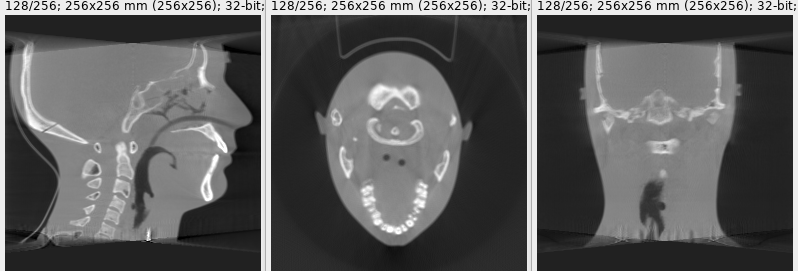
\includegraphics[width=0.8\textwidth]{reconstruction}
                        \caption{Ricostruzione del fantoccio presentato in \texttt{Figura \ref{fig:skull-phantom}}
                        utilizzando la procedura rtkfdk. Immagine a sinistra, una sezione del piano sagittale; immagine centrale, una sezione del piano coronale; immagine destra, una sezione del piano trasverso. }
                        \label{fig:reconstruction}
                        
                    \end{figure}
            
            
            
    \chapter{Creazione Package Python}
        \section{RTK-Handler}
            \subsection{Scopo}
                \par 
                    Inizialmente tutte le procedure di generazione geometria e di normalizzazione descritte nelle sezioni 12,13 <TODO!! unmagnet links> si sono implementate all'interno di moduli Python completamente separati tra loro....
                    <TODO>
                    RTK-handler automates the Normalization process according to (2) and creates the .xml geometry according to this:\newline
                    \url{http://www.openrtk.org/Doxygen/geometry.pdf}\newline\newline
                    It also provides an interface to the rtkfdk procedure in order to get a reconstruction from:
                    \begin{itemize}
                    \item Normalized stack:
                    Simply reconstructs with rtkfdk.
                    \newline
                    \\OR
                    \item Non normalized .tiff set:
                        It performs an auto-normalization and than reconstructs with rtkfdk.\newline
                        \end{itemize}
                        The binary rtkfdk is simply executed by Python from the \textit{/path\_of\_RTK-bin/RTK-bin/bin} 
                        folder by choosing the .mha projections stack and the .xml geometry file directly by the folder structure generated by RTK-handler and asking the rest of the parameters directly from the user. 
            \subsection{Architettura}
            \subsection{Utilizzo}
            \subsection{Estensione}
            \subsection{Utilizzi futuri}
            
    \chapter{Risultati e Conclusioni}
        \subsection{Risultati}
        \subsection{Conclusioni}



\newpage
\begin{thebibliography}{1}
    \bibitem{zeng-tomos}
        Gengsheng, Z. L. (2010). Basic Principles of Tomography. In Springer (Ed.), \textit{Medical Image Reconstruction: A Conceptual Tutorial}.
        
    \bibitem{openrtk-website}
        \url{http://www.openrtk.org/}
    
    \bibitem{itk-website}
        \url{https://itk.org/}
    
    \bibitem{conventional-tomography}
        Littleton, J.T. "Conventional Tomography". A History of the Radiological Sciences (PDF). American Roentgen Ray Society. Retrieved 11 January 2014.
    
    \bibitem{vallebona-ricordo}
        Franco Bistolfi, Alessandro Vallebona 1899-1987. Ricordo di un grande radiologo e del suo contributo allo sviluppo delle scienze radiologiche (PDF), in Fisica in Medicina, nº 2, 2005, pp. 115-123.
        
    \bibitem{vallebona-pensiero}
        Vallebona A. - Gli ottanta anni della radiologia medica in Liguria. Atti dell’Accademia Ligure di Scienze e Lettere, XXXI: 18-46,1974
        
    \bibitem{thomas-edison-brain}
        \url{https://www.researchgate.net/publication/18576763_Thomas_Edison's_attempts_at_radiography_of_the_brain_1896}
        
    \bibitem{hounsfield-nobel-lecture}
        Godfrey N. Hounsfield - Nobel Lecture, 8 December 1979
        
    \bibitem{vallebona-difesa}
        \url{http://www.fisicamedica.it/museo_virtuale/02_sezioni/articoli/data/Vallebona%20difesa.pdf}
        
    \bibitem{nobel-debate}
        Riddle of the Nobel debate - Science 04 Jan 1980: Vol. 207, Issue 4426, pp. 37-38
        
    \bibitem{hounsfield-autobiografia}
        \url{https://www.nobelprize.org/nobel_prizes/medicine/laureates/1979/hounsfield-bio.html}
    
    \bibitem{-j-gnu-docs}
        \url{https://www.gnu.org/software/make/manual/html_node/Parallel.html}
        
    \bibitem{wiki-rtk}
        \url{wiki.openrtk.org}
        
    \bibitem{rtk-users-proj-offset}
        \url{http://public.kitware.com/pipermail/rtk-users/2014-December/000344.html}
        
    \bibitem{simplertk-wiki}
        \url{http://wiki.openrtk.org/index.php/SimpleRTK}
        
    \bibitem{imagej-3dio-plugin}
        \url{http://ij-plugins.sourceforge.net/plugins/3d-io/index.html}
    
    \bibitem{lambert-beer}
        \url{https://en.wikipedia.org/wiki/Beer%E2%80%93Lambert_law}
        
    \bibitem{pyexcel-docs}
        \url{http://pyexcel.readthedocs.io/en/latest/generated/pyexcel.Sheet.html#pyexcel.Sheet}
        
    \bibitem{python-list}
        \url{https://docs.python.org/3/library/stdtypes.html#lists}
        
    \bibitem{float-python}
        \url{https://docs.python.org/3/library/functions.html#float}
        
    \bibitem{input-python}
        \url{https://docs.python.org/3/library/functions.html#input}
        
    \bibitem{projections-reader}
        \url{http://www.openrtk.org/Doxygen/classrtk_1_1ProjectionsReader.html}
    
    \bibitem{sitk-readimage}
        \url{https://itk.org/SimpleITKDoxygen/html/classitk_1_1simple_1_1ImageFileReader.html}
    
    \bibitem{sitk-estractor}
        \url{https://itk.org/SimpleITKDoxygen/html/classitk_1_1simple_1_1ExtractImageFilter.html#details}
    
    \bibitem{python-range}
        \url{https://docs.python.org/3/library/stdtypes.html#range}
        
    \bibitem{sitk-log}
        \url{https://itk.org/SimpleITKDoxygen/html/classitk_1_1simple_1_1LogImageFilter.html#details}
        
    \bibitem{sitk-joinseries}
        \url{https://itk.org/SimpleITKDoxygen/html/classitk_1_1simple_1_1JoinSeriesImageFilter.html#details}
        
    \bibitem{sitk-paste}
        \url{https://itk.org/SimpleITKDoxygen/html/classitk_1_1simple_1_1PasteImageFilter.html#details}
        
    \end{thebibliography}
\end{document}
